\subsection{Datierung}

Insgesamt liegen 101 unterschiedliche Zeitintervalle (\texttt{RANGE}) vor, welche insgesamt 21 Perioden zugeordnet wurden. Für die Betrachtung eines groben zeitlichen Trends sind 21 Perioden jedoch zu viele (und 101 Zeitintervalle erst recht). 
In \texttt{an\_6} bis \texttt{an\_8} wurden die Perioden und Ranges näher betrachtet mit der Absicht, die Einteilung zu vergröbern. Hierbei wurde jedoch ein Problem offensichtlich: die Funde überlappen sich teilweise in ihrer Datierung, sodass keine klaren Grenzen gezogen werden können, s. \autoref{fig:timeline}

\begin{figure}[H]
    \centering
    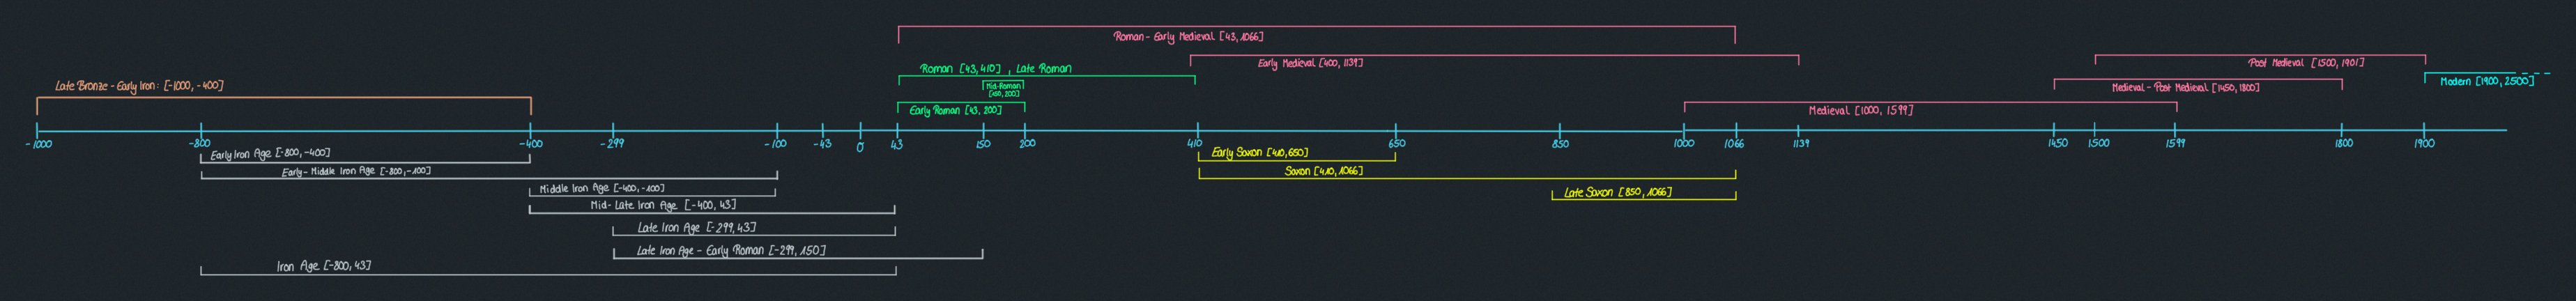
\includegraphics[width=\textwidth]{docs/latex/attachments/ab-project_timeline.png}
    \caption{Eine Skizze der im Datensatz definierten Perioden}
    \label{fig:timeline}
\end{figure}

Wenn ein Fund z.B. auf das Intervall zwischen -299 und 150 datiert wurde, ein anderer aber auf zwischen 43 und 200 kann man weder bei 150 noch bei 43 eine Grenze ziehen.
Daher werden die Funde wie in \autoref{fig:timeline_highlighted} grob in vier Zeitkategorien eingeteilt, um eine Betrachtung der Größenentwicklung über die Zeit zu ermöglichen. 
Die Überlappungen wurden in dieser Einteilung möglichst gering gehalten, lassen sich aber natürlich nicht ganz ausschließen.

\begin{figure}[H]
    \centering
    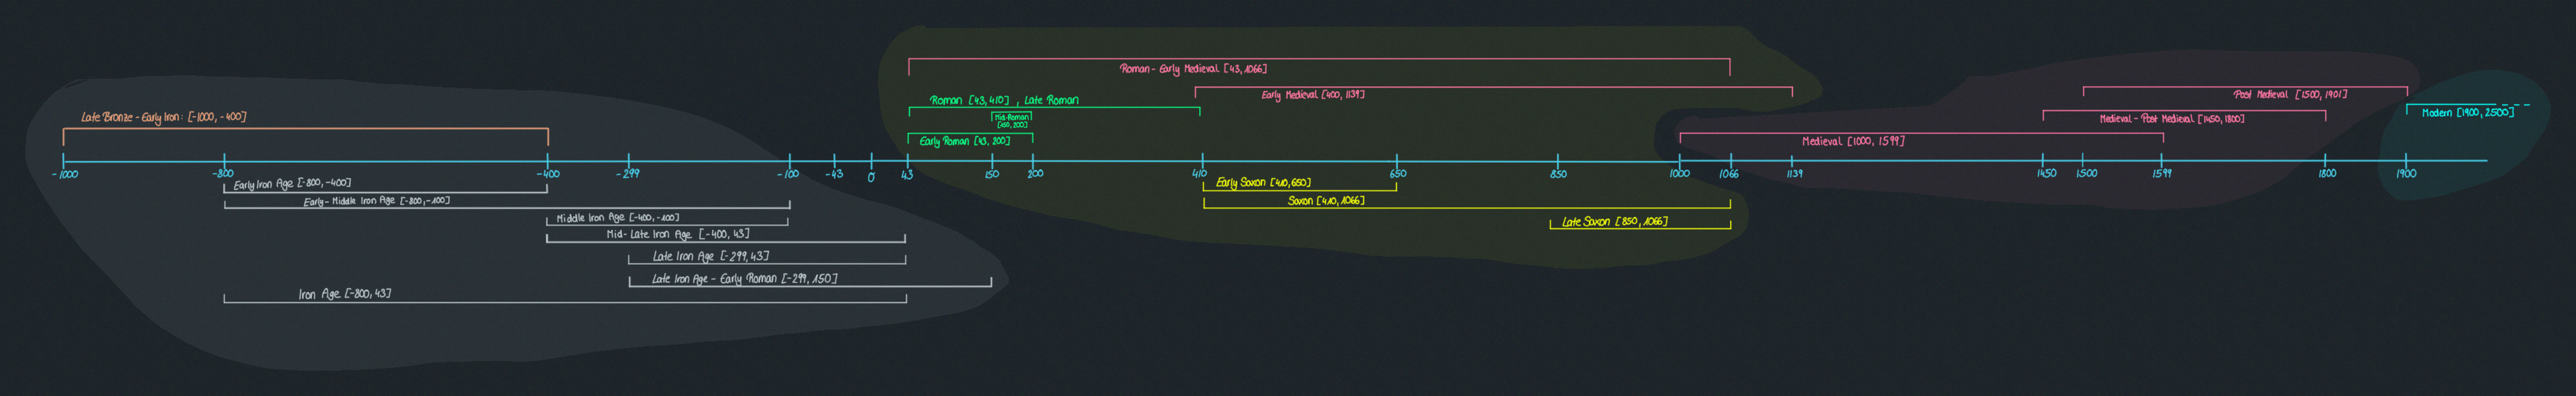
\includegraphics[width=\textwidth]{docs/latex/attachments/ab-project_timeline-highlighted.png}
    \caption{Die gewählten vier Gruppen wurden farblich hervorgehoben}
    \label{fig:timeline_highlighted}
\end{figure}

In \texttt{an\_7} wurde das \texttt{PERIOD}-Attribut der Funde entsprechend aktualisiert.

Figure 2.4 zeigt die Mengen der Funde und Messungen für alle Knochentypen pro Periode.